%!TEX root = ../main.tex

\chapter{Experiment\label{chap:experiment}}

The experiment was performed with two X500 \ac{UAV}s, each of them equipped with a Prophesee EVK4 event-based camera, one with a 2.5mm f/1.6
fish eye lens with an \ac{FOV} of 93.5 degrees and the second one with Entaniya 1.07mm f/2.8 fish eye lens with an \ac{FOV} of 280 degrees.
Each UAV is also equipped with a Basler camera with a fish eye lens, to provide normal video signal that is recorded alongside the event stream
from the event-based camera.
Both cameras are connected to the onboard Intel NUC computer running the ROS system, on which all the processing is done during the flight. Both 
\ac{UAV}s are also equipped with a \ac{RTK} module, which is used to localize the \ac{UAV}, and is used as ground truth data for the pose estimation.
The UVDAR blinking frequencies $\mathcal{F} = \{4.0, 2.0, 1.\overline{3}, 1.0\}$ (in kHz) were defined, where each of the arms were blinking at its assigned
frequency.
The measurements were collected during the \ac{MRS} Camp in Temešvár in August 2025, the \ac{UAV}s can be seen on \reffig{fig:uav33_37}.
\begin{figure}[H]
	\centering
	\subfloat[UAV33] {
	  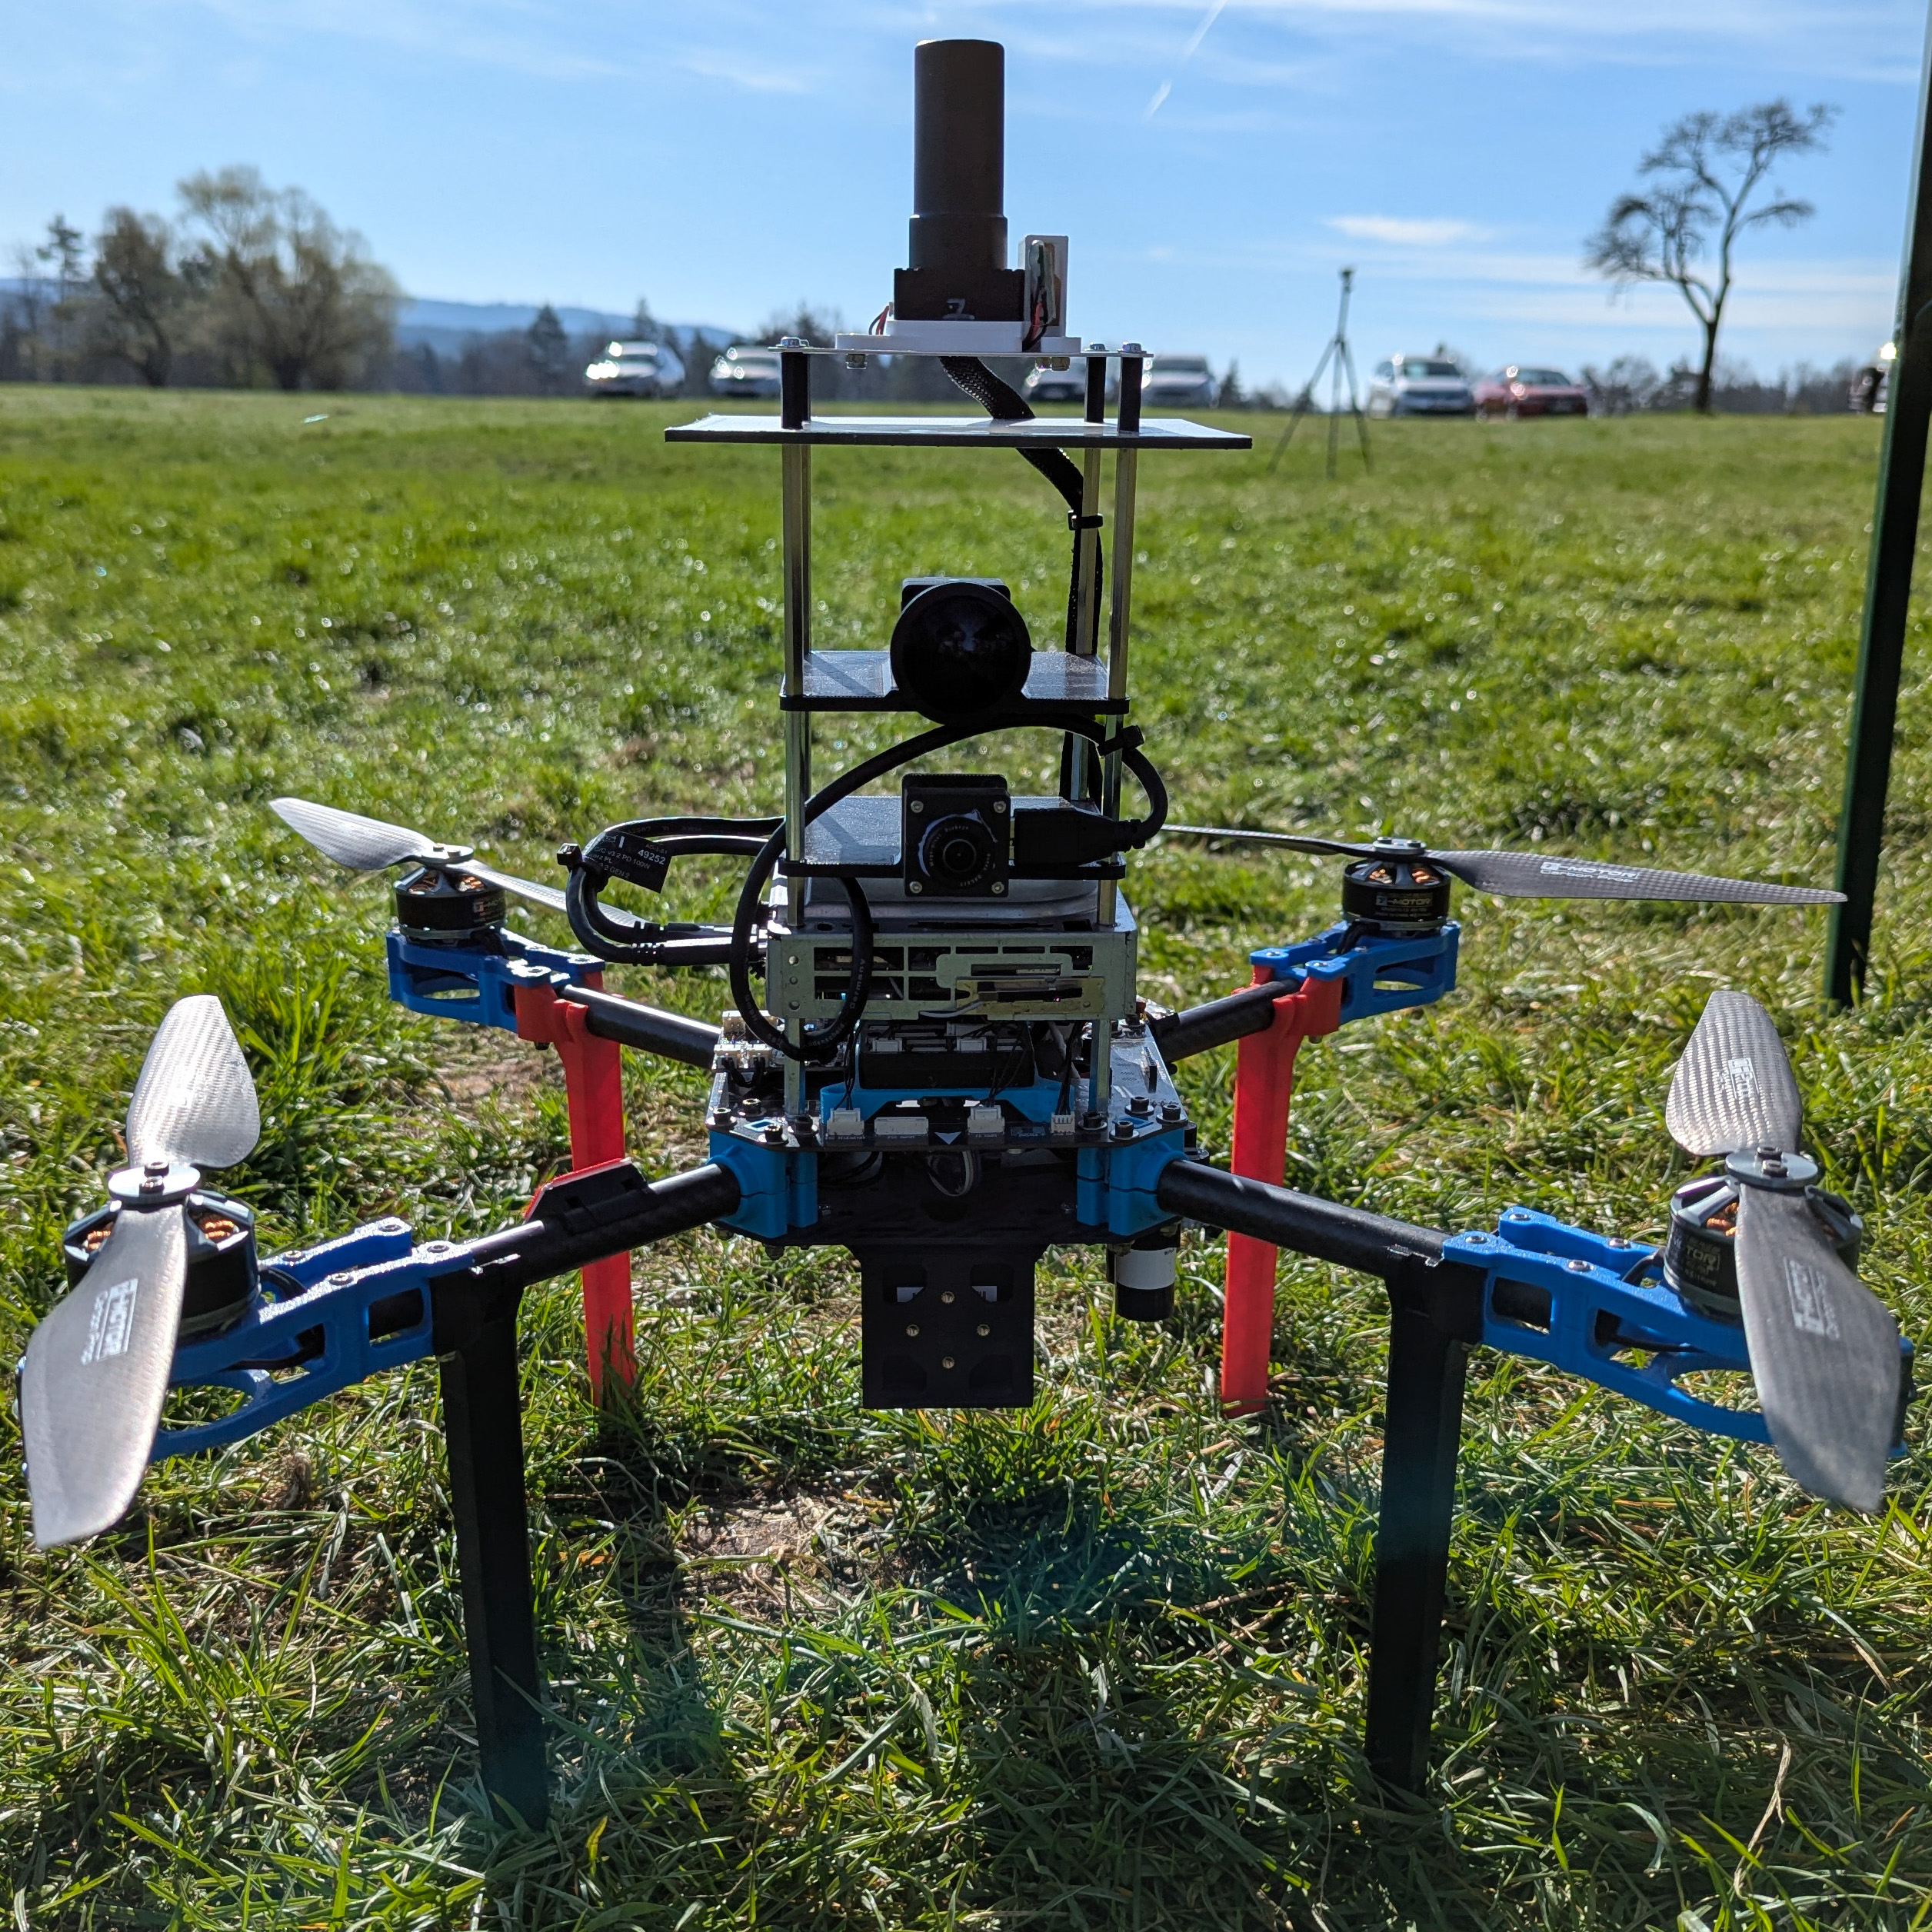
\includegraphics[width=0.4\textwidth]{./fig/photos/uav33.jpg}
	  \label{fig:uav33}
	}
	\subfloat[UAV37] {
	  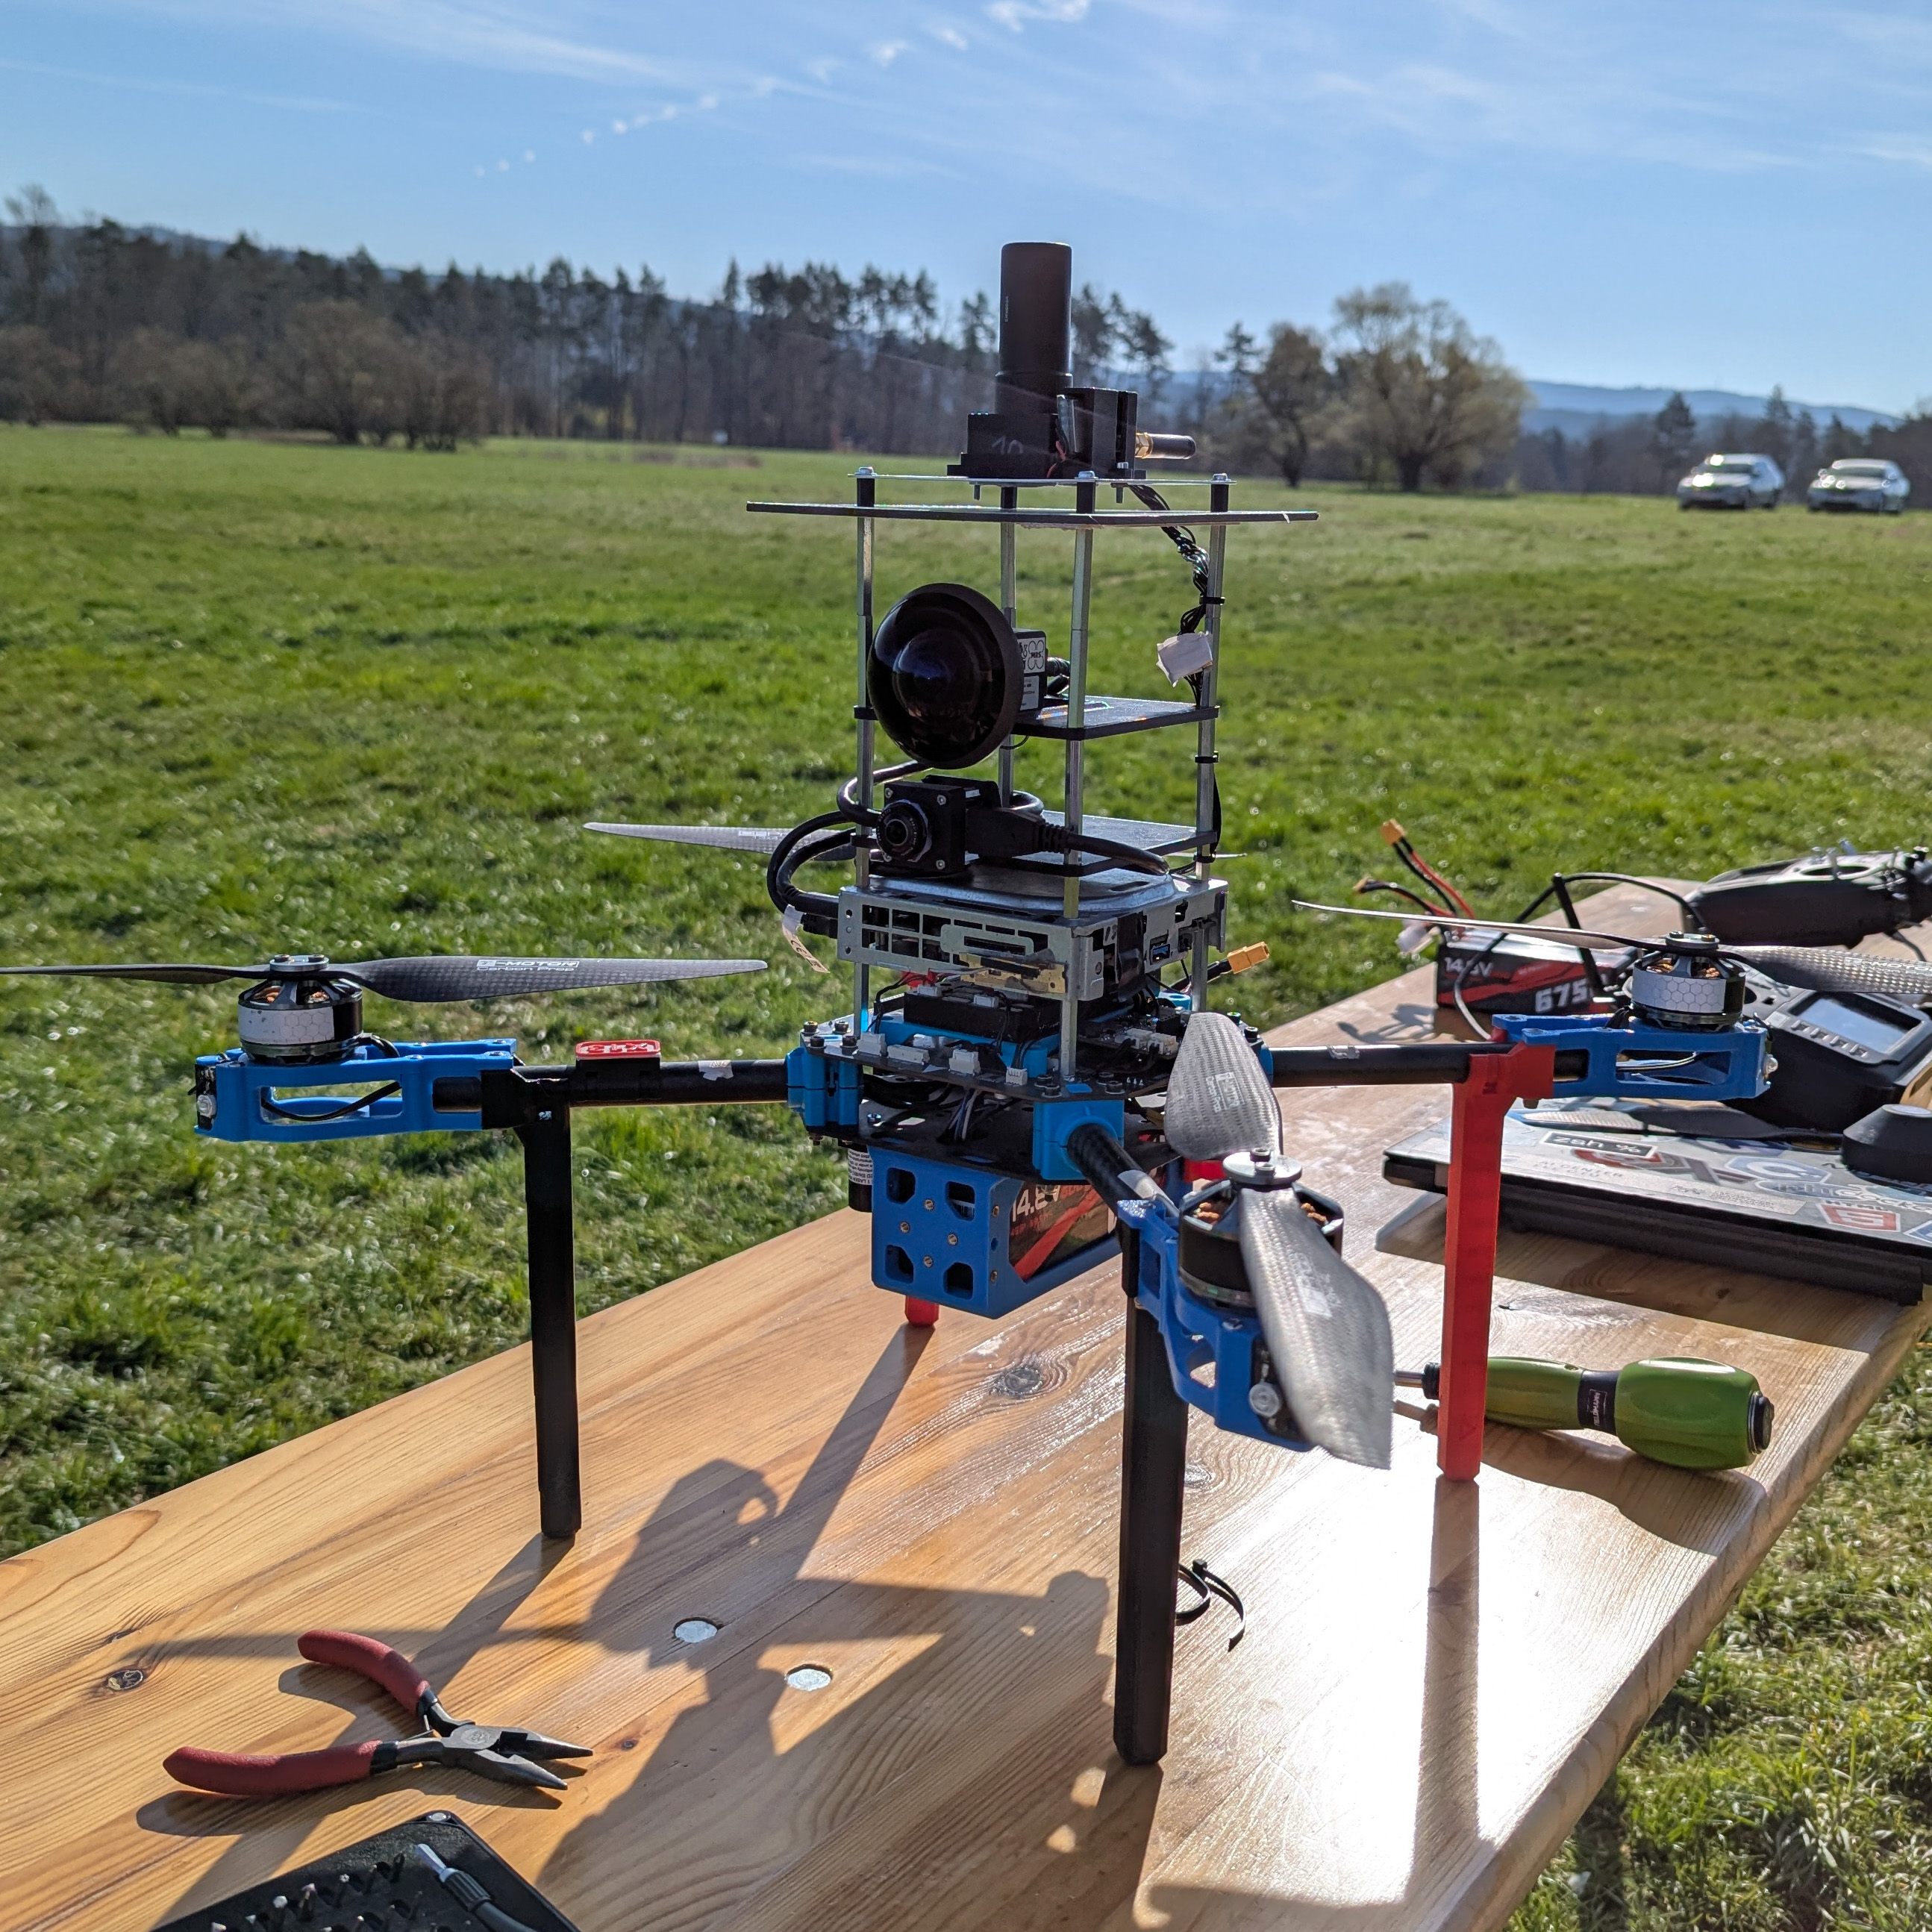
\includegraphics[width=0.4\textwidth]{./fig/photos/uav37.jpg}
	  \label{fig:uav37}
	}
	\caption{
		Two X500 UAVs, UAV33 on \reffig{fig:uav33} and UAV37 on \reffig{fig:uav37}.
  }
	\label{fig:uav33_37}
\end{figure}
Two pilots manually controlled the \ac{UAV}s, systematically varying the distance and angles between them to generate diverse measurement data during the experiment. All in-flight data, including sensor measurements and camera streams, we recorden in a \ac{ROS} bag file for subsequent analysis
in a simulated environment. In addition, raw event stream data from the event-based camera was also recorded and saved. The camera view from the UAV33
can be seen on \reffig{fig:exp1}

\begin{figure}[H]
	\centering
	\subfloat[Event-based camera output] {
	  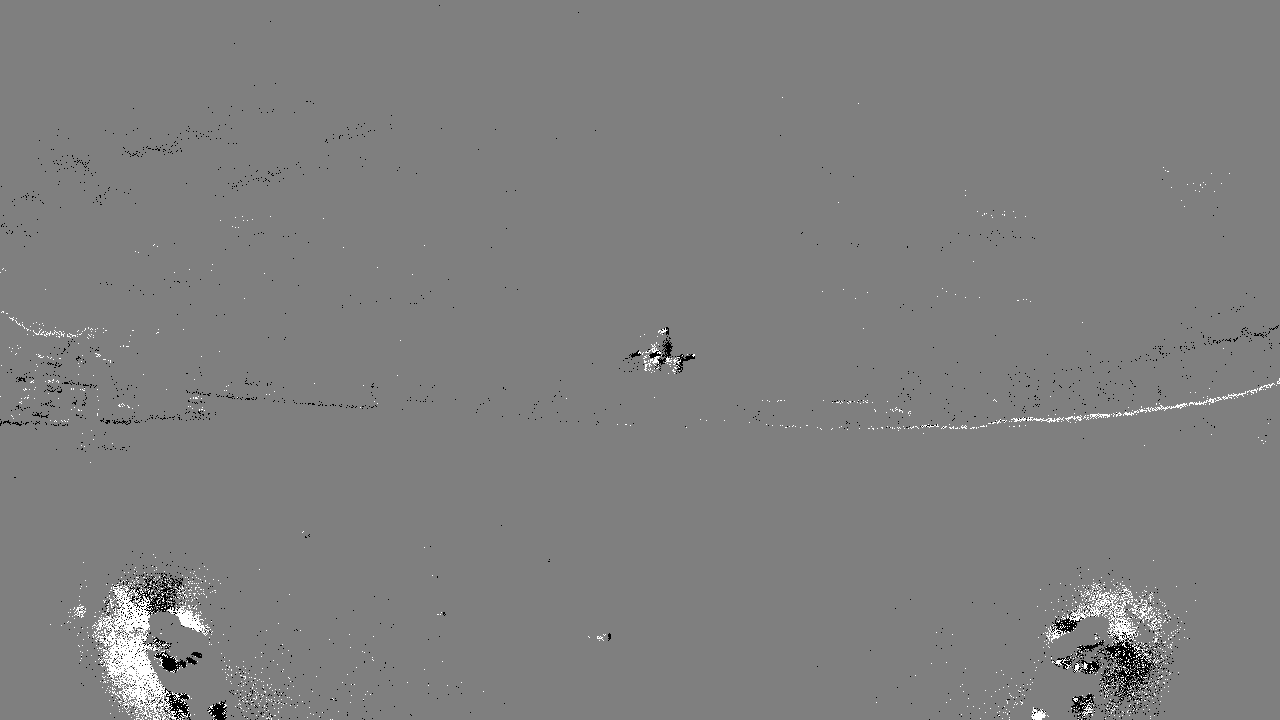
\includegraphics[width=0.50\textwidth]{./fig/photos/uav33_event.png}
	  \label{fig:exp1_event}
	}
	\subfloat[Basler camera output] {
	  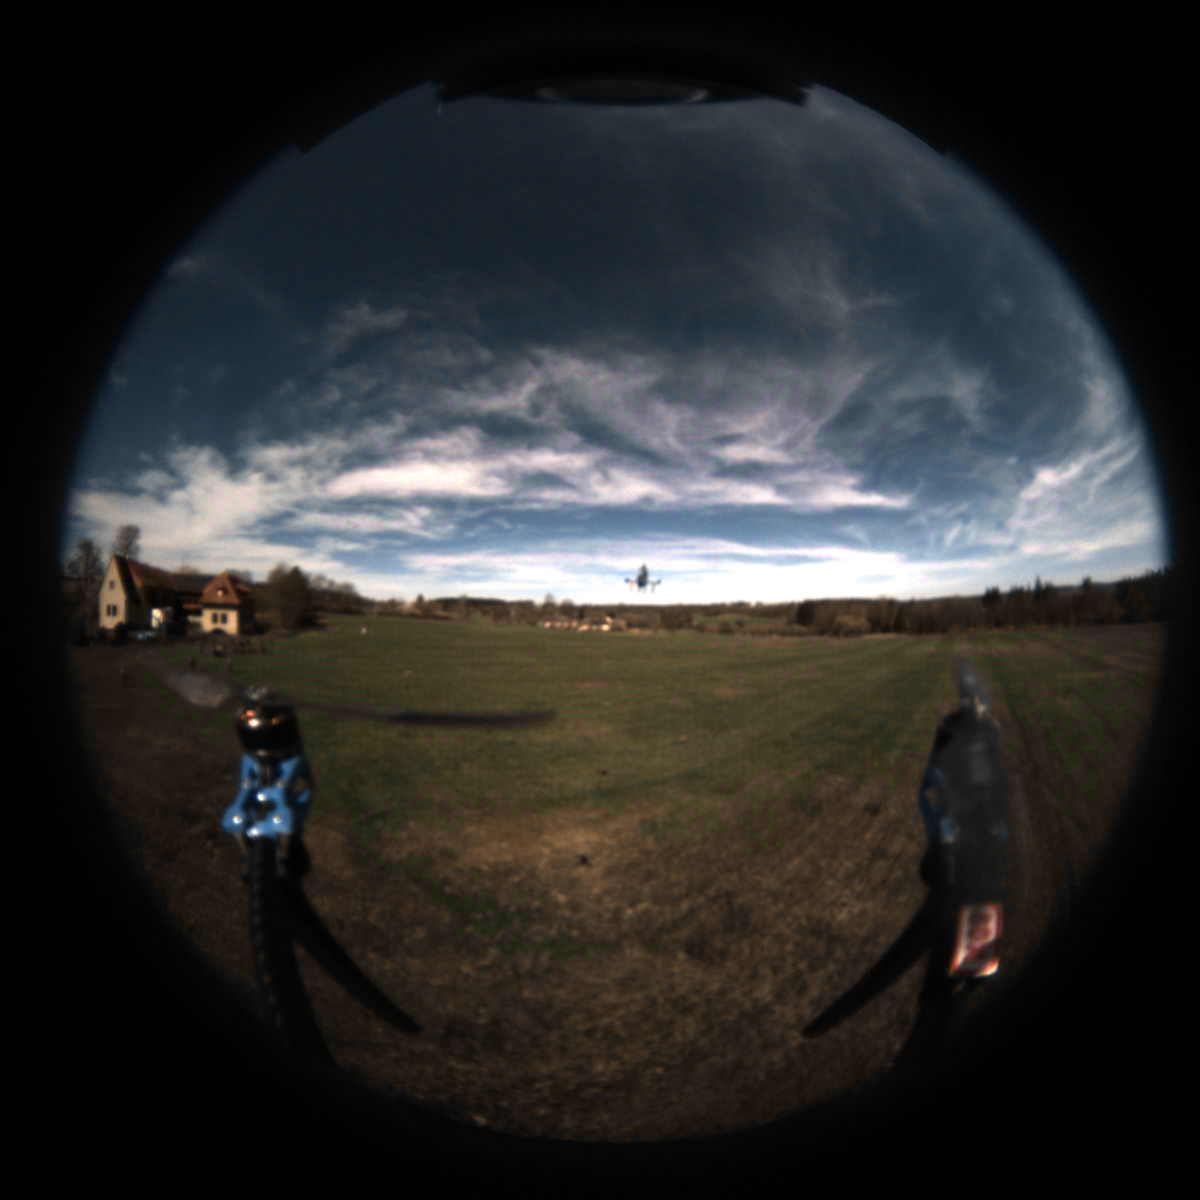
\includegraphics[width=0.282\textwidth]{./fig/photos/uav33_basler.png}
	  \label{fig:exp1_basler}
	}
	\caption{
		The view of the experiment from UAV33, with event data on \reffig{fig:exp1_event} and Basler camera view on \reffig{fig:exp1_basler}.
  }
	\label{fig:exp1}
\end{figure}

\todo{SHOW MEASURED DATA FROM RQT}

\todo{SHOW GNSS/ESTIMATION DIFFERENCES}

\todo{SHOW THE RVIZ/RQTPLOT VISUALIZATION PIPELINE}
